\documentclass[11pt]{article}
\usepackage[textwidth=18.0cm, textheight=23.0cm, top=2.0cm]{geometry}
\usepackage{pst-all}
\usepackage{amssymb}
\usepackage{tikz}
\usepackage{underscore}\begin{document}
\pagestyle{empty}


ClassName: \underline{\textbf{Class_07.2bp-16}}
\par
BinSize: \underline{\textbf{100 × 100}}
\par
ReduceSize: \underline{\textbf{100 × 100}}
\par
TypeNum: \underline{\textbf{39}}
\par
Num: \underline{\textbf{40}}
\par
OutS: \underline{\textbf{120000}}
\par
InS: \underline{\textbf{90896}}
\par
Rate: \underline{\textbf{0.757}}
\par
UB: \underline{\textbf{12}}
\par
LB0: \underline{\textbf{12}}
\par
LB: \underline{\textbf{12}}
\par
LBWithCut: \underline{\textbf{12}}
\par
NodeCut: \underline{\textbf{0}}
\par
ExtendedNodeCnt: \underline{\textbf{1}}
\par
GenNodeCnt: \underline{\textbf{1}}
\par
PrimalNode: \underline{\textbf{0}}
\par
ColumnCount: \underline{\textbf{12}}
\par
TotalCutCount: \underline{\textbf{0}}
\par
RootCutCount: \underline{\textbf{0}}
\par
LPSolverCnt: \underline{\textbf{1}}
\par
PricingSolverCnt: \underline{\textbf{0}}
\par
BranchAndBoundNum: \underline{\textbf{1}}
\par
isOpt: \underline{\textbf{true}}
\par
TimeOnInitSolution: \underline{\textbf{120.010 s}}
\par
TimeOnPrimal: \underline{\textbf{0.000 s}}
\par
TimeOnPricing: \underline{\textbf{0.000 s}}
\par
TimeOnRmp: \underline{\textbf{0.079 s}}
\par
TotalTime: \underline{\textbf{120.135 s}}
\par
\newpage


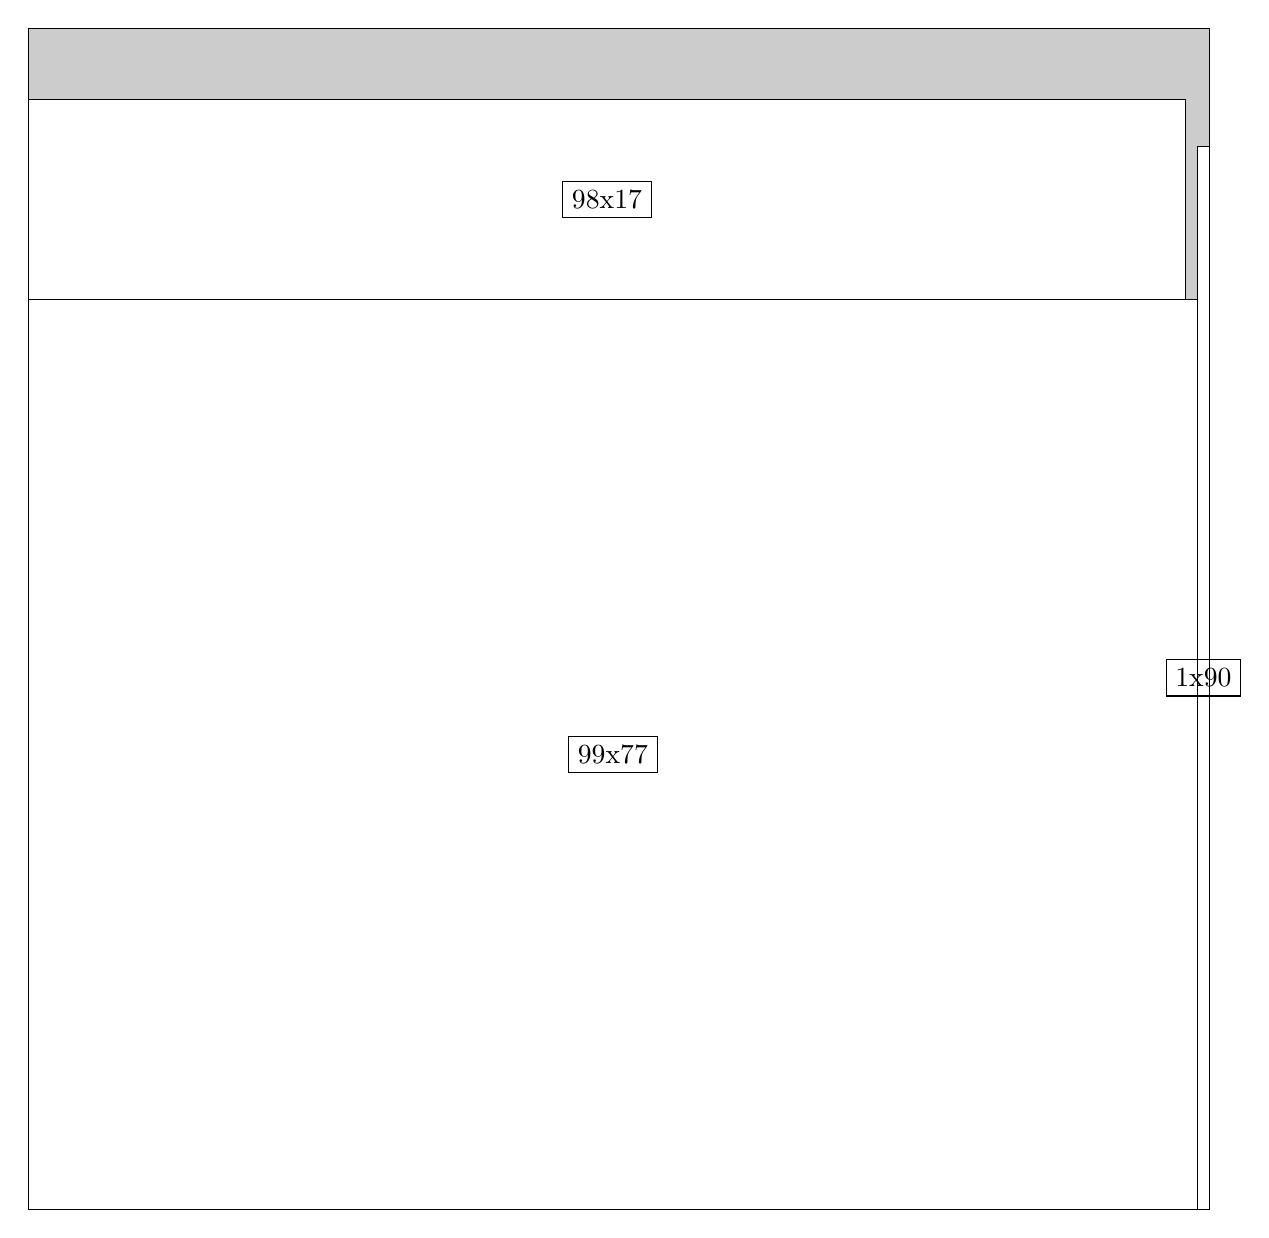
\begin{tikzpicture}[shorten >=1pt,scale=1.0,every node/.style={scale=1.0},->]
\tikzstyle{vertex}=[circle,fill=black!25,minimum size=14pt,inner sep=0pt]
\filldraw[fill=gray!40!white, draw=black] (0,0) rectangle (15.0,15.0);
\foreach \name/\x/\y/\w/\h in {99x77/0.0/0.0/14.85/11.549999999999999,1x90/14.85/0.0/0.15/13.5,98x17/0.0/11.549999999999999/14.7/2.55}
\filldraw[fill=white!40!white, draw=black] (\x,\y) rectangle node[draw] (\name) {\name} ++(\w,\h);
\end{tikzpicture}


w =99 , h =77 , x =0 , y =0 , v =7623
\par
w =1 , h =90 , x =99 , y =0 , v =90
\par
w =98 , h =17 , x =0 , y =77 , v =1666
\par
\newpage


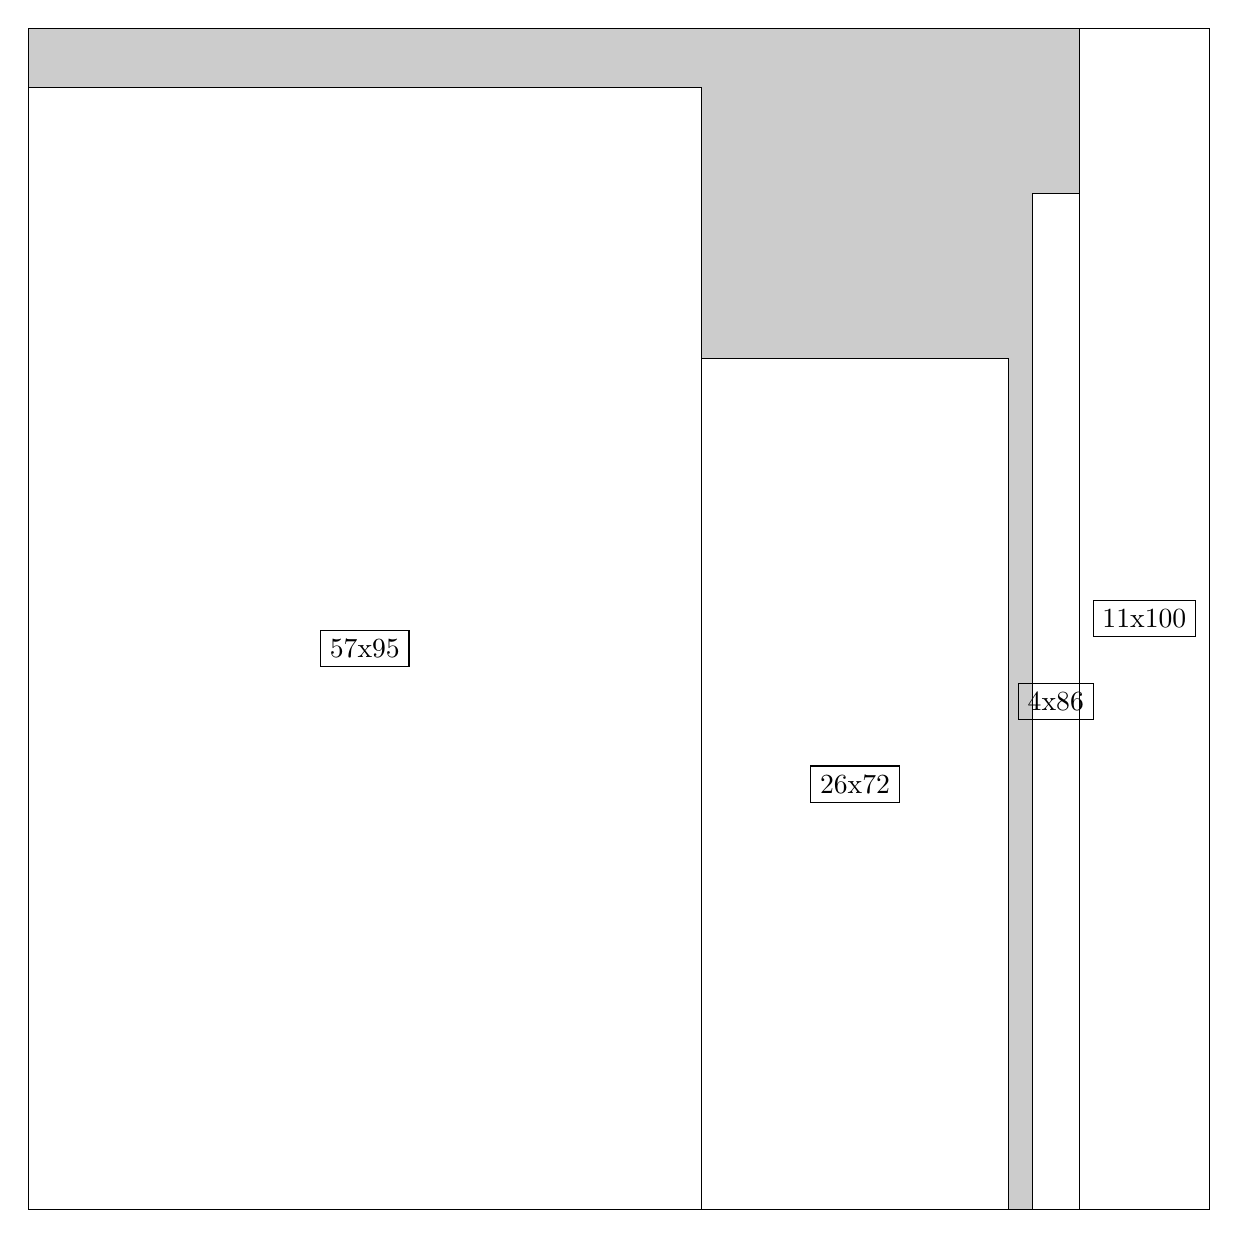
\begin{tikzpicture}[shorten >=1pt,scale=1.0,every node/.style={scale=1.0},->]
\tikzstyle{vertex}=[circle,fill=black!25,minimum size=14pt,inner sep=0pt]
\filldraw[fill=gray!40!white, draw=black] (0,0) rectangle (15.0,15.0);
\foreach \name/\x/\y/\w/\h in {57x95/0.0/0.0/8.549999999999999/14.25,26x72/8.549999999999999/0.0/3.9/10.799999999999999,11x100/13.35/0.0/1.65/15.0,4x86/12.75/0.0/0.6/12.9}
\filldraw[fill=white!40!white, draw=black] (\x,\y) rectangle node[draw] (\name) {\name} ++(\w,\h);
\end{tikzpicture}


w =57 , h =95 , x =0 , y =0 , v =5415
\par
w =26 , h =72 , x =57 , y =0 , v =1872
\par
w =11 , h =100 , x =89 , y =0 , v =1100
\par
w =4 , h =86 , x =85 , y =0 , v =344
\par
\newpage


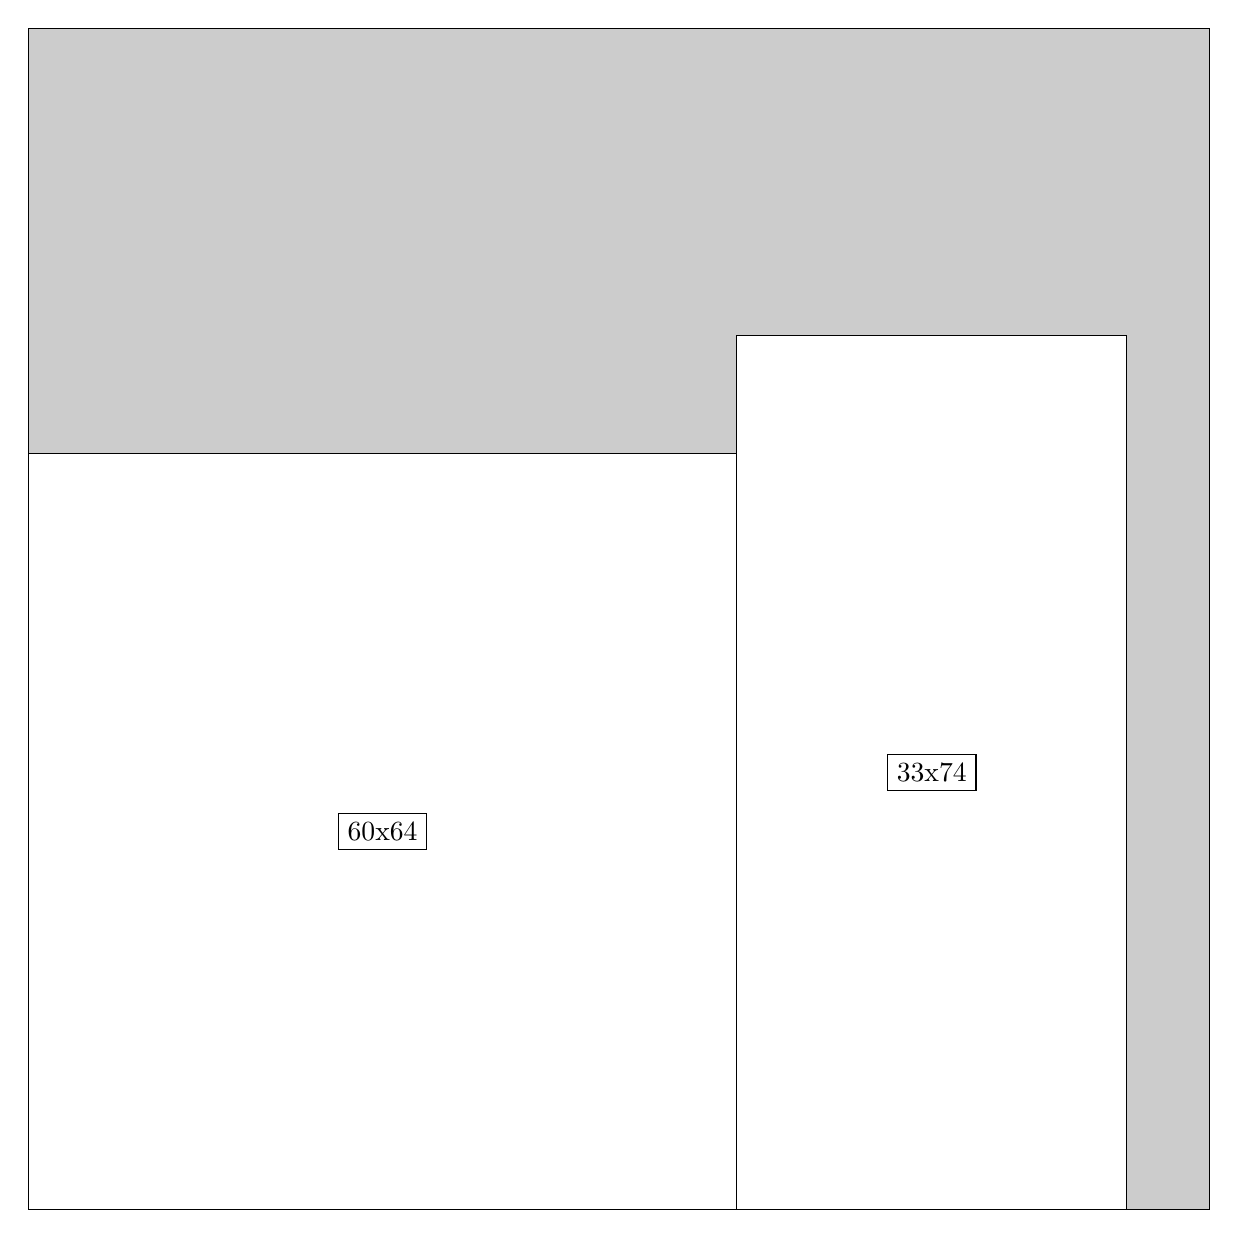
\begin{tikzpicture}[shorten >=1pt,scale=1.0,every node/.style={scale=1.0},->]
\tikzstyle{vertex}=[circle,fill=black!25,minimum size=14pt,inner sep=0pt]
\filldraw[fill=gray!40!white, draw=black] (0,0) rectangle (15.0,15.0);
\foreach \name/\x/\y/\w/\h in {60x64/0.0/0.0/9.0/9.6,33x74/9.0/0.0/4.95/11.1}
\filldraw[fill=white!40!white, draw=black] (\x,\y) rectangle node[draw] (\name) {\name} ++(\w,\h);
\end{tikzpicture}


w =60 , h =64 , x =0 , y =0 , v =3840
\par
w =33 , h =74 , x =60 , y =0 , v =2442
\par
\newpage


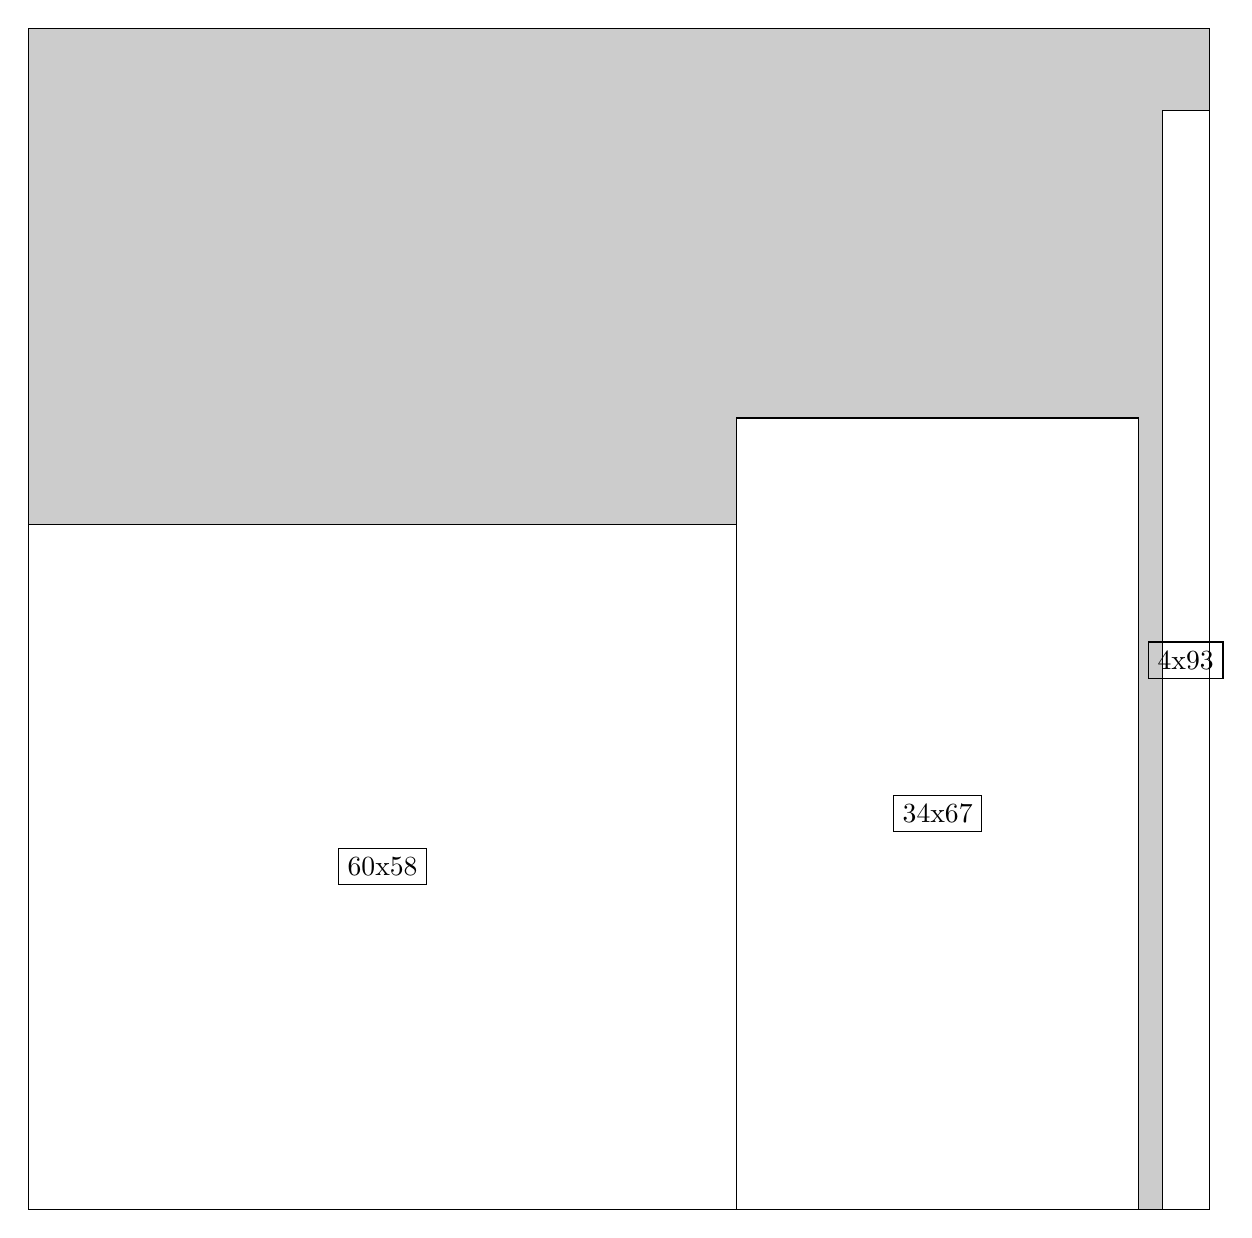
\begin{tikzpicture}[shorten >=1pt,scale=1.0,every node/.style={scale=1.0},->]
\tikzstyle{vertex}=[circle,fill=black!25,minimum size=14pt,inner sep=0pt]
\filldraw[fill=gray!40!white, draw=black] (0,0) rectangle (15.0,15.0);
\foreach \name/\x/\y/\w/\h in {60x58/0.0/0.0/9.0/8.7,34x67/9.0/0.0/5.1/10.049999999999999,4x93/14.399999999999999/0.0/0.6/13.95}
\filldraw[fill=white!40!white, draw=black] (\x,\y) rectangle node[draw] (\name) {\name} ++(\w,\h);
\end{tikzpicture}


w =60 , h =58 , x =0 , y =0 , v =3480
\par
w =34 , h =67 , x =60 , y =0 , v =2278
\par
w =4 , h =93 , x =96 , y =0 , v =372
\par
\newpage


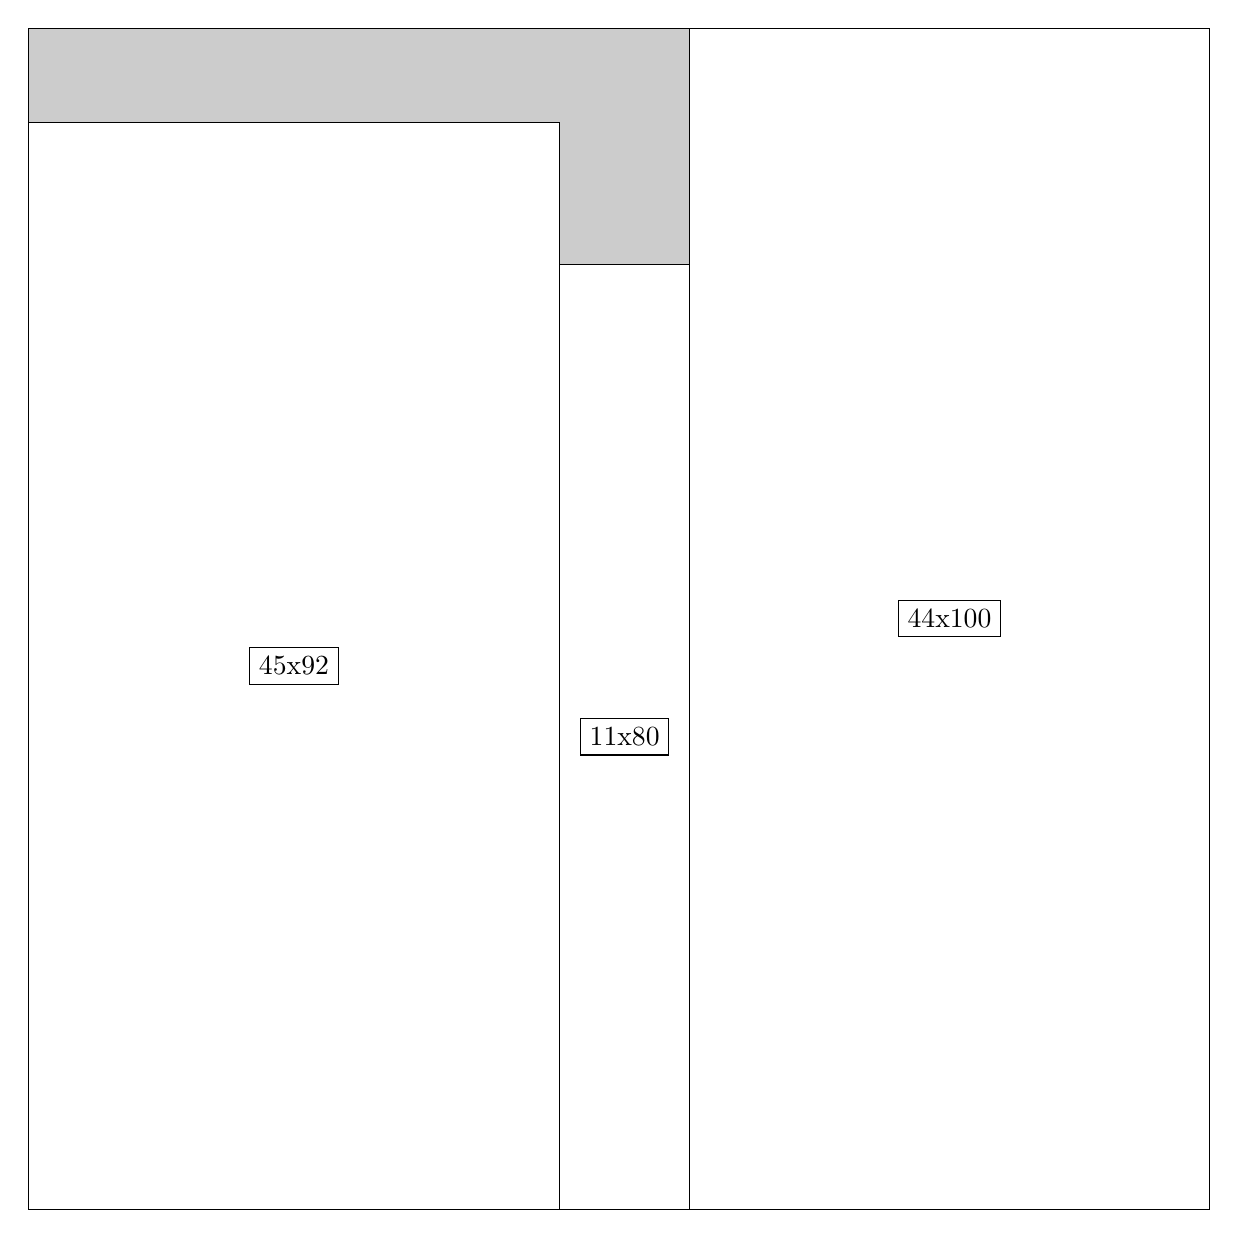
\begin{tikzpicture}[shorten >=1pt,scale=1.0,every node/.style={scale=1.0},->]
\tikzstyle{vertex}=[circle,fill=black!25,minimum size=14pt,inner sep=0pt]
\filldraw[fill=gray!40!white, draw=black] (0,0) rectangle (15.0,15.0);
\foreach \name/\x/\y/\w/\h in {44x100/8.4/0.0/6.6/15.0,45x92/0.0/0.0/6.75/13.799999999999999,11x80/6.75/0.0/1.65/12.0}
\filldraw[fill=white!40!white, draw=black] (\x,\y) rectangle node[draw] (\name) {\name} ++(\w,\h);
\end{tikzpicture}


w =44 , h =100 , x =56 , y =0 , v =4400
\par
w =45 , h =92 , x =0 , y =0 , v =4140
\par
w =11 , h =80 , x =45 , y =0 , v =880
\par
\newpage


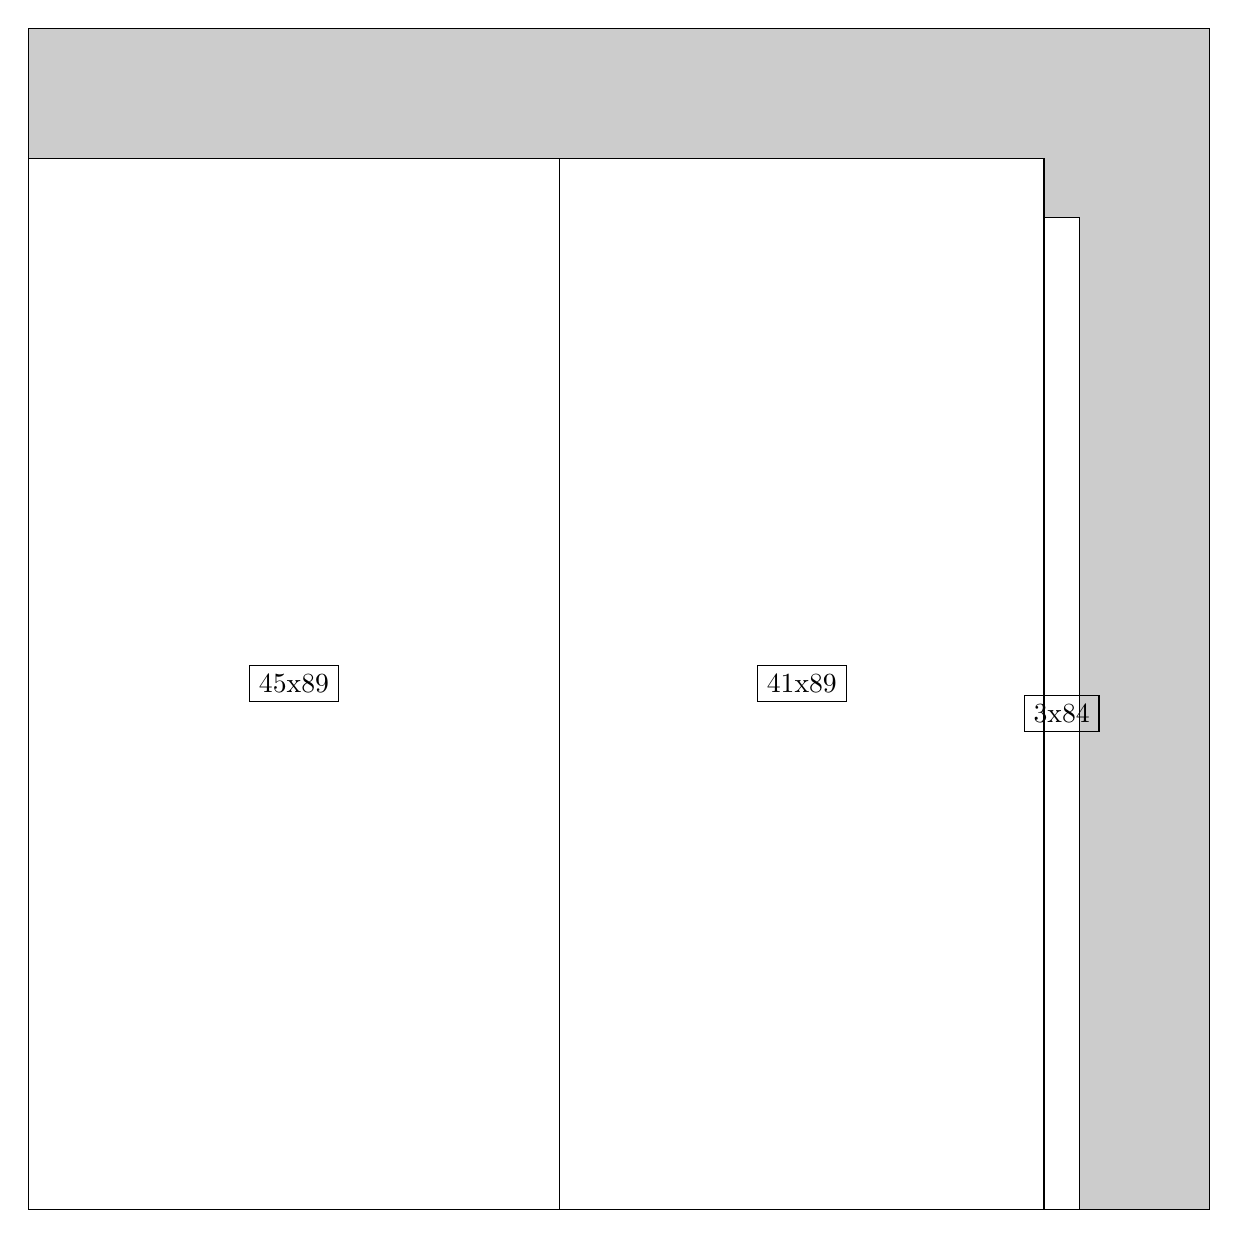
\begin{tikzpicture}[shorten >=1pt,scale=1.0,every node/.style={scale=1.0},->]
\tikzstyle{vertex}=[circle,fill=black!25,minimum size=14pt,inner sep=0pt]
\filldraw[fill=gray!40!white, draw=black] (0,0) rectangle (15.0,15.0);
\foreach \name/\x/\y/\w/\h in {45x89/0.0/0.0/6.75/13.35,41x89/6.75/0.0/6.1499999999999995/13.35,3x84/12.9/0.0/0.44999999999999996/12.6}
\filldraw[fill=white!40!white, draw=black] (\x,\y) rectangle node[draw] (\name) {\name} ++(\w,\h);
\end{tikzpicture}


w =45 , h =89 , x =0 , y =0 , v =4005
\par
w =41 , h =89 , x =45 , y =0 , v =3649
\par
w =3 , h =84 , x =86 , y =0 , v =252
\par
\newpage


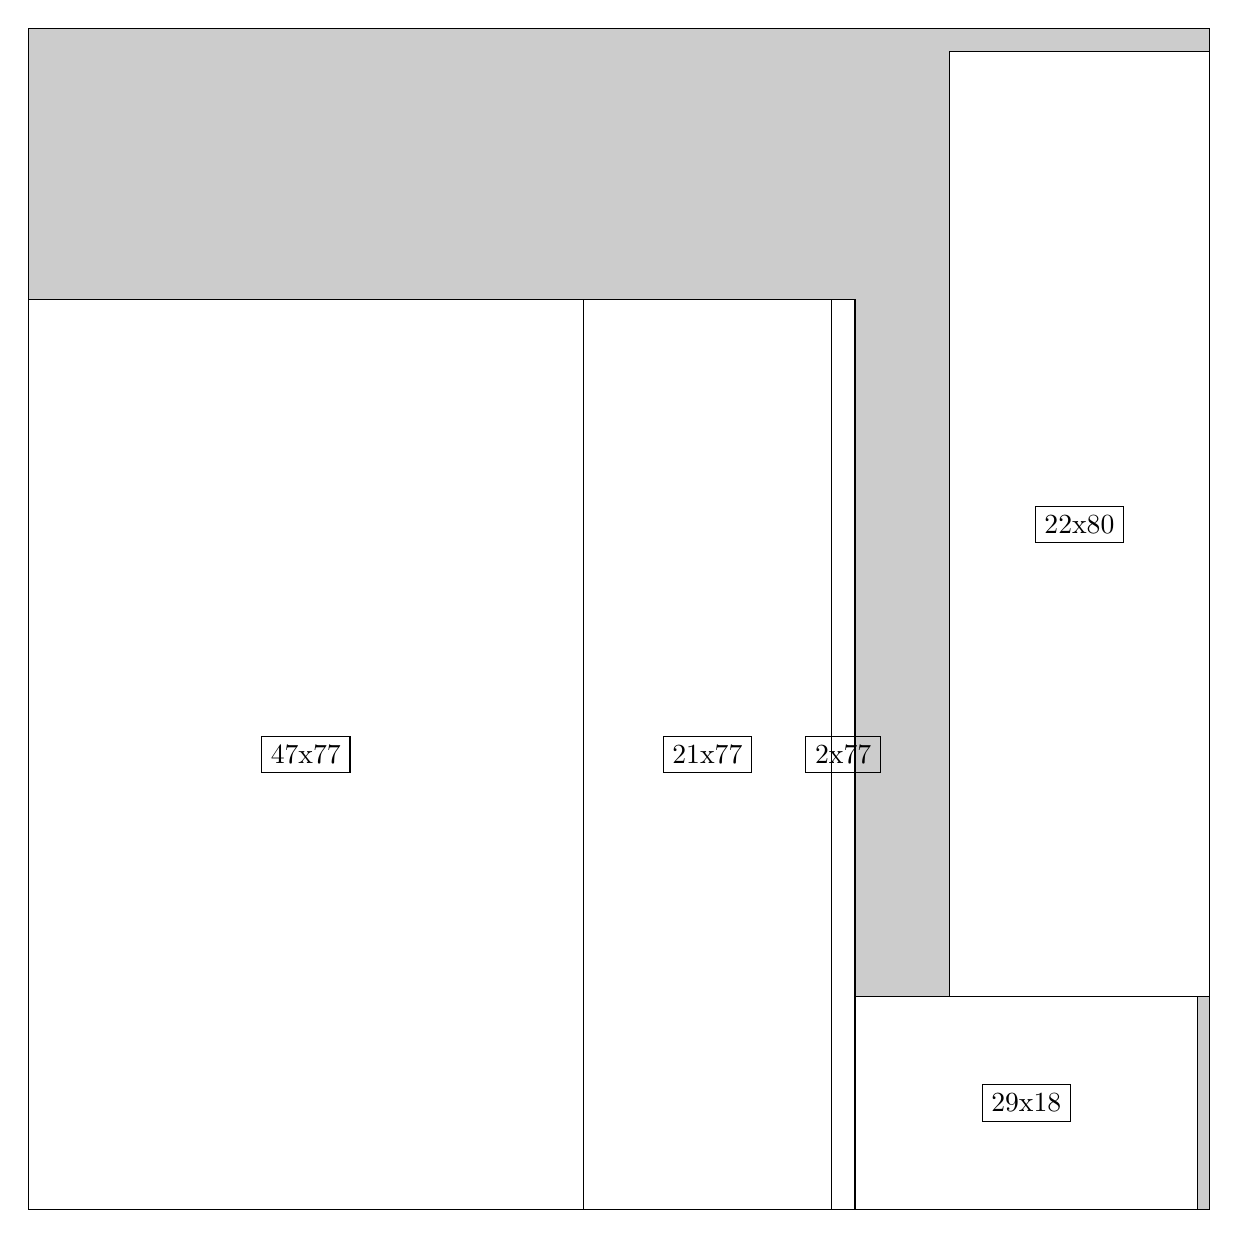
\begin{tikzpicture}[shorten >=1pt,scale=1.0,every node/.style={scale=1.0},->]
\tikzstyle{vertex}=[circle,fill=black!25,minimum size=14pt,inner sep=0pt]
\filldraw[fill=gray!40!white, draw=black] (0,0) rectangle (15.0,15.0);
\foreach \name/\x/\y/\w/\h in {47x77/0.0/0.0/7.05/11.549999999999999,22x80/11.7/2.6999999999999997/3.3/12.0,21x77/7.05/0.0/3.15/11.549999999999999,29x18/10.5/0.0/4.35/2.6999999999999997,2x77/10.2/0.0/0.3/11.549999999999999}
\filldraw[fill=white!40!white, draw=black] (\x,\y) rectangle node[draw] (\name) {\name} ++(\w,\h);
\end{tikzpicture}


w =47 , h =77 , x =0 , y =0 , v =3619
\par
w =22 , h =80 , x =78 , y =18 , v =1760
\par
w =21 , h =77 , x =47 , y =0 , v =1617
\par
w =29 , h =18 , x =70 , y =0 , v =522
\par
w =2 , h =77 , x =68 , y =0 , v =154
\par
\newpage


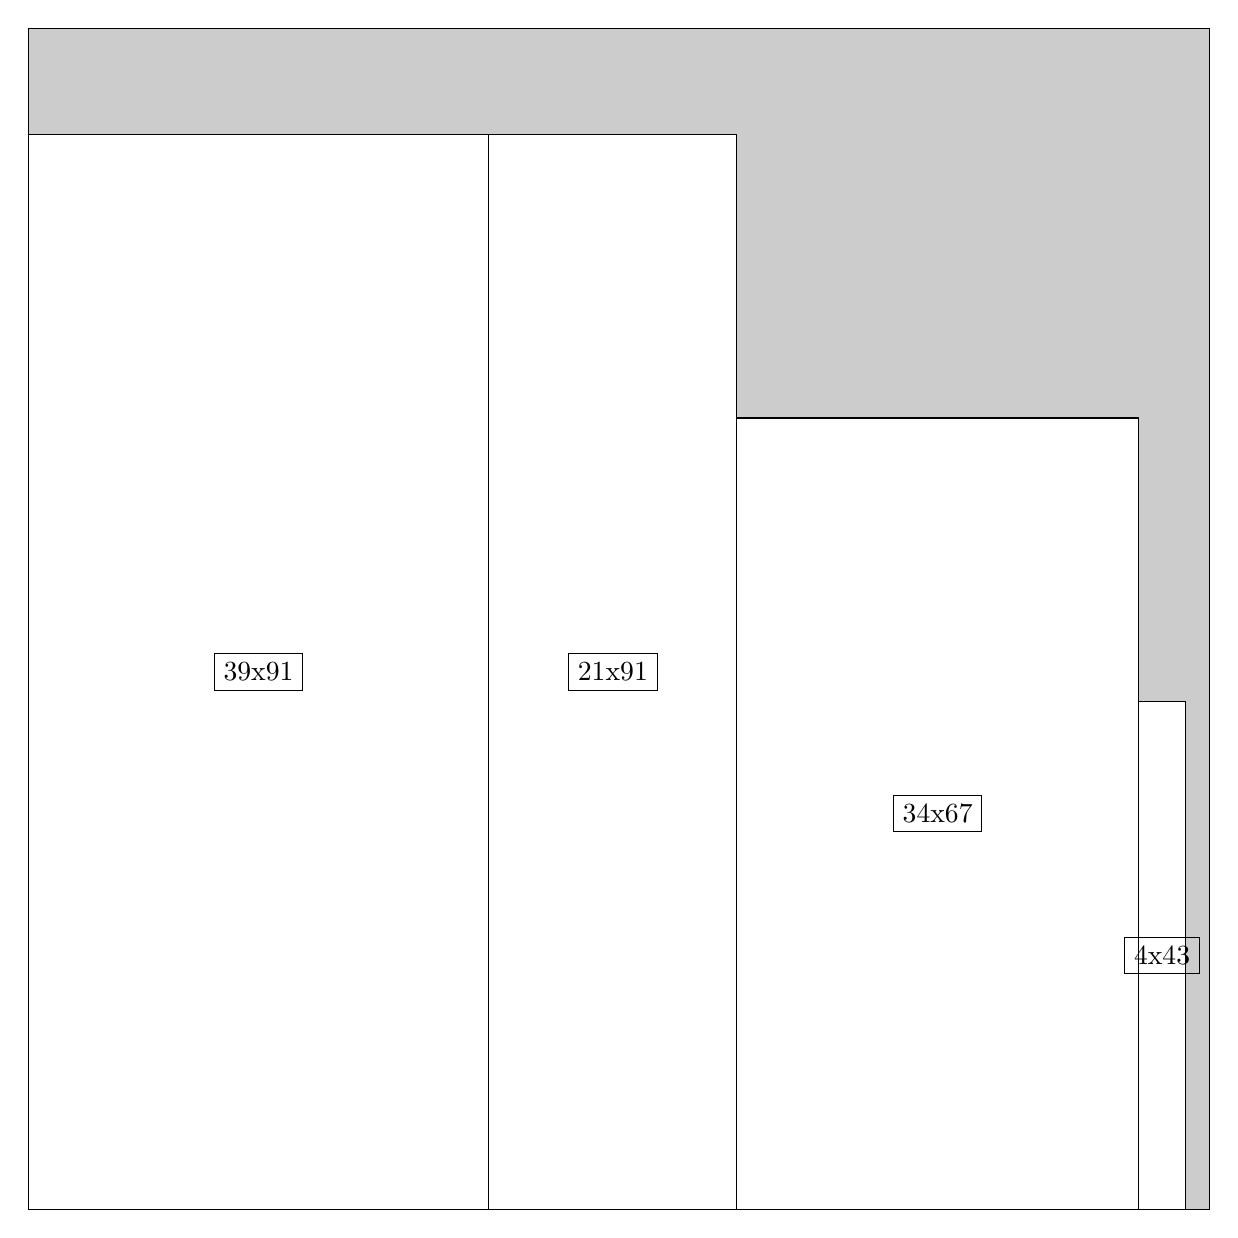
\begin{tikzpicture}[shorten >=1pt,scale=1.0,every node/.style={scale=1.0},->]
\tikzstyle{vertex}=[circle,fill=black!25,minimum size=14pt,inner sep=0pt]
\filldraw[fill=gray!40!white, draw=black] (0,0) rectangle (15.0,15.0);
\foreach \name/\x/\y/\w/\h in {39x91/0.0/0.0/5.85/13.65,34x67/9.0/0.0/5.1/10.049999999999999,21x91/5.85/0.0/3.15/13.65,4x43/14.1/0.0/0.6/6.45}
\filldraw[fill=white!40!white, draw=black] (\x,\y) rectangle node[draw] (\name) {\name} ++(\w,\h);
\end{tikzpicture}


w =39 , h =91 , x =0 , y =0 , v =3549
\par
w =34 , h =67 , x =60 , y =0 , v =2278
\par
w =21 , h =91 , x =39 , y =0 , v =1911
\par
w =4 , h =43 , x =94 , y =0 , v =172
\par
\newpage


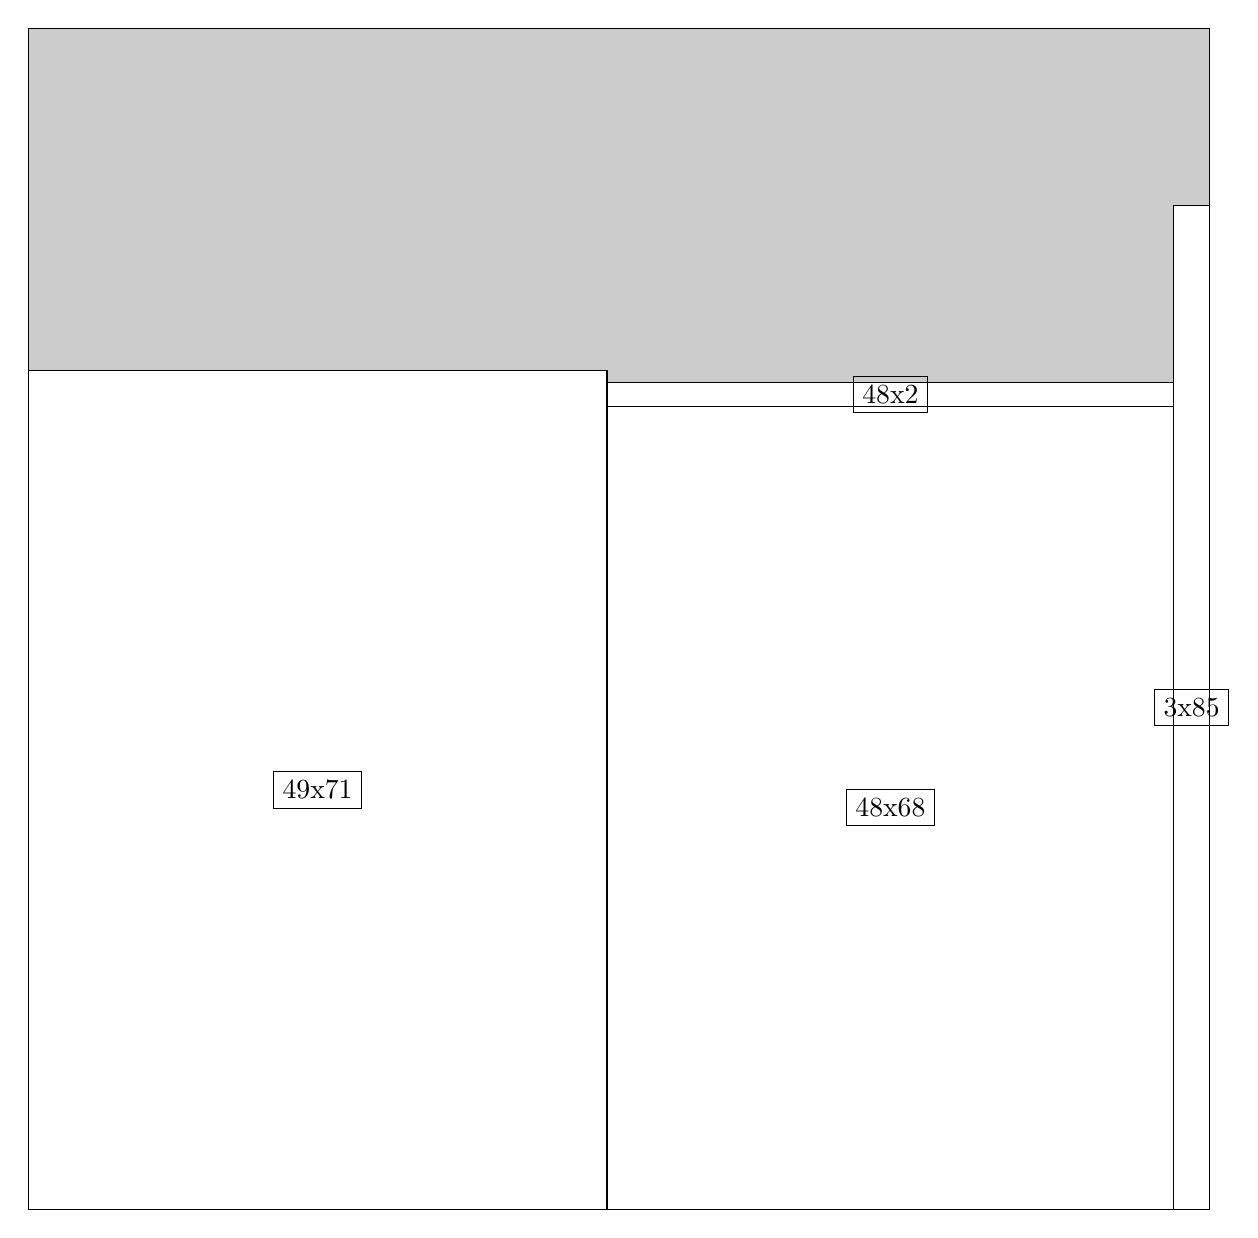
\begin{tikzpicture}[shorten >=1pt,scale=1.0,every node/.style={scale=1.0},->]
\tikzstyle{vertex}=[circle,fill=black!25,minimum size=14pt,inner sep=0pt]
\filldraw[fill=gray!40!white, draw=black] (0,0) rectangle (15.0,15.0);
\foreach \name/\x/\y/\w/\h in {49x71/0.0/0.0/7.35/10.65,48x68/7.35/0.0/7.199999999999999/10.2,3x85/14.549999999999999/0.0/0.44999999999999996/12.75,48x2/7.35/10.2/7.199999999999999/0.3}
\filldraw[fill=white!40!white, draw=black] (\x,\y) rectangle node[draw] (\name) {\name} ++(\w,\h);
\end{tikzpicture}


w =49 , h =71 , x =0 , y =0 , v =3479
\par
w =48 , h =68 , x =49 , y =0 , v =3264
\par
w =3 , h =85 , x =97 , y =0 , v =255
\par
w =48 , h =2 , x =49 , y =68 , v =96
\par
\newpage


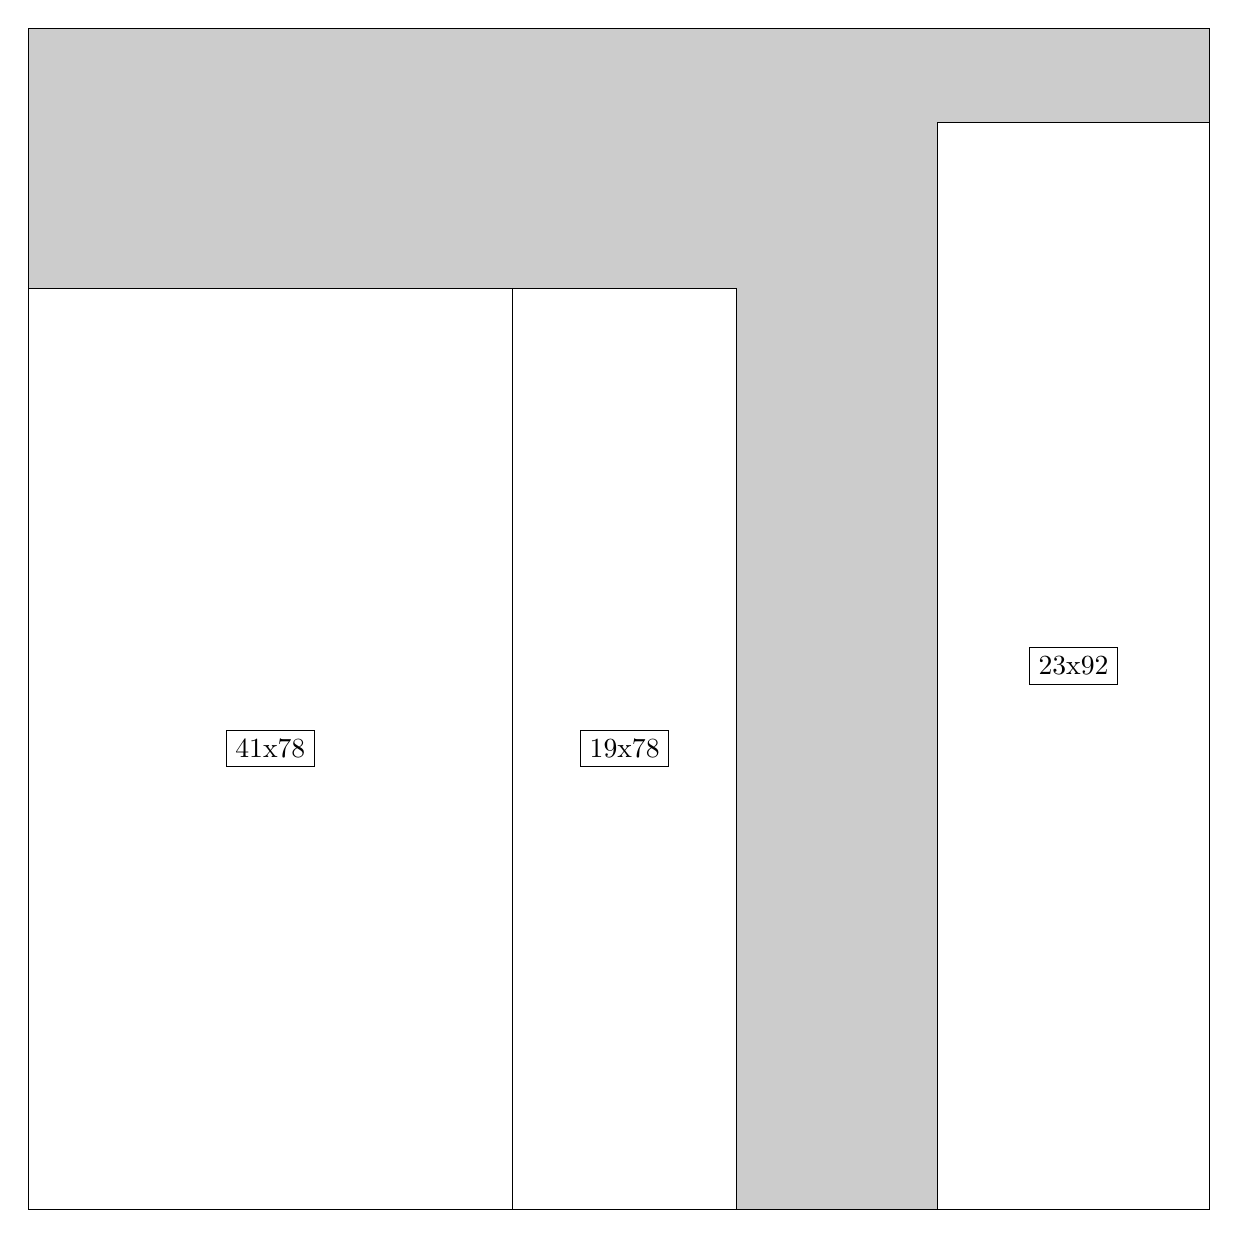
\begin{tikzpicture}[shorten >=1pt,scale=1.0,every node/.style={scale=1.0},->]
\tikzstyle{vertex}=[circle,fill=black!25,minimum size=14pt,inner sep=0pt]
\filldraw[fill=gray!40!white, draw=black] (0,0) rectangle (15.0,15.0);
\foreach \name/\x/\y/\w/\h in {41x78/0.0/0.0/6.1499999999999995/11.7,23x92/11.549999999999999/0.0/3.4499999999999997/13.799999999999999,19x78/6.1499999999999995/0.0/2.85/11.7}
\filldraw[fill=white!40!white, draw=black] (\x,\y) rectangle node[draw] (\name) {\name} ++(\w,\h);
\end{tikzpicture}


w =41 , h =78 , x =0 , y =0 , v =3198
\par
w =23 , h =92 , x =77 , y =0 , v =2116
\par
w =19 , h =78 , x =41 , y =0 , v =1482
\par
\newpage


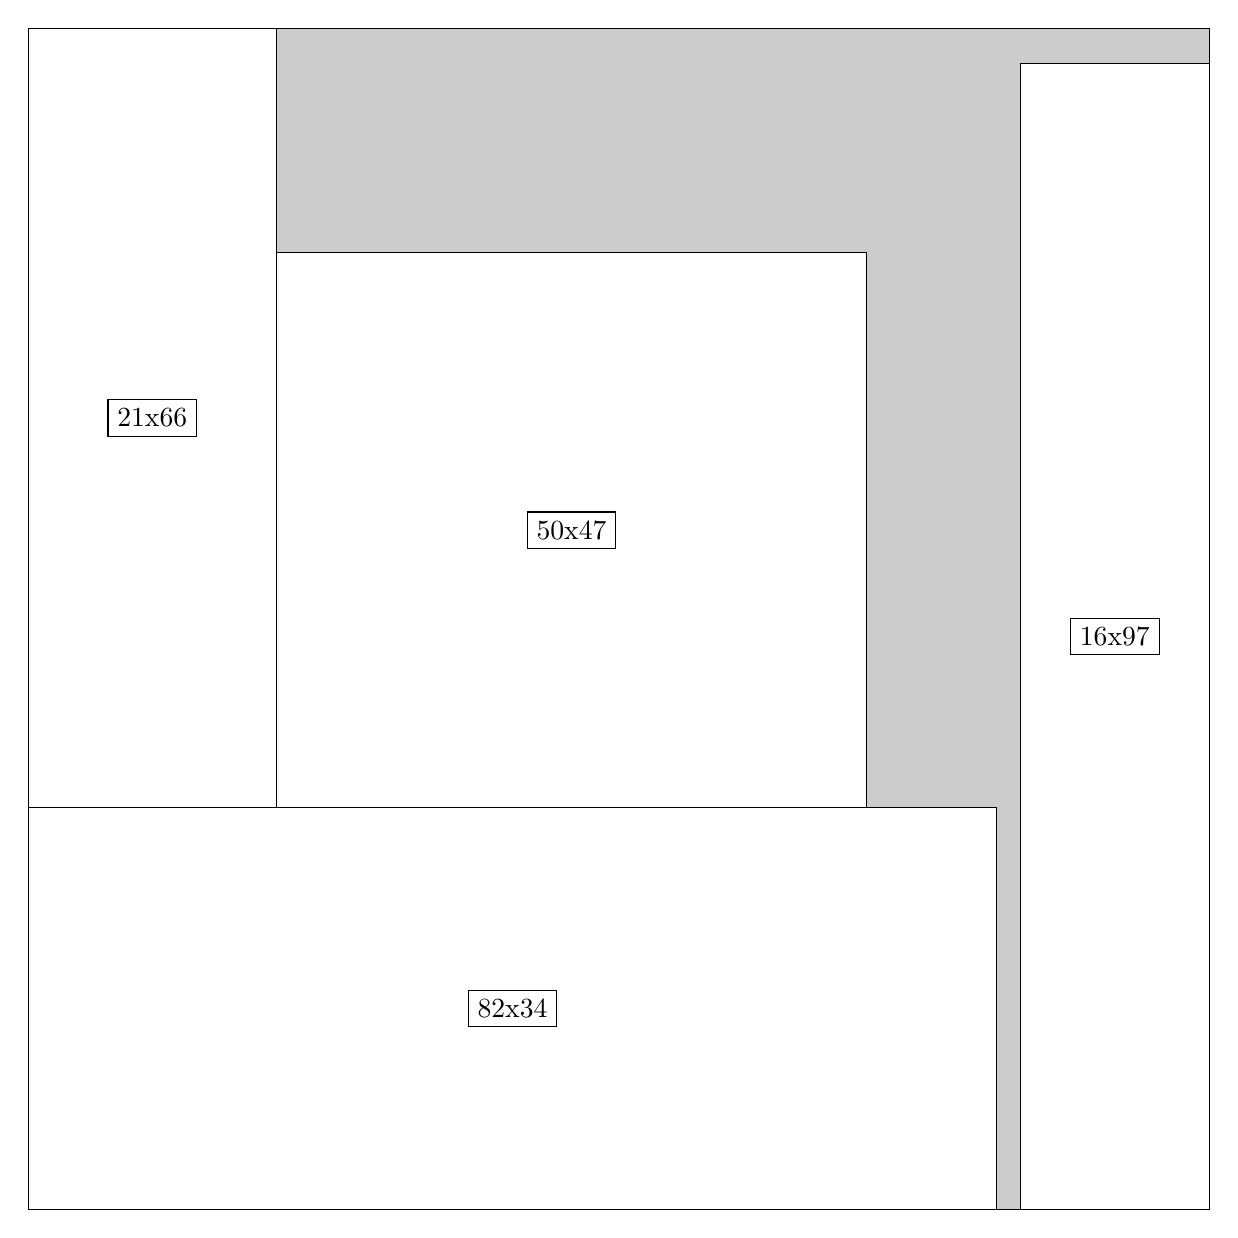
\begin{tikzpicture}[shorten >=1pt,scale=1.0,every node/.style={scale=1.0},->]
\tikzstyle{vertex}=[circle,fill=black!25,minimum size=14pt,inner sep=0pt]
\filldraw[fill=gray!40!white, draw=black] (0,0) rectangle (15.0,15.0);
\foreach \name/\x/\y/\w/\h in {82x34/0.0/0.0/12.299999999999999/5.1,50x47/3.15/5.1/7.5/7.05,16x97/12.6/0.0/2.4/14.549999999999999,21x66/0.0/5.1/3.15/9.9}
\filldraw[fill=white!40!white, draw=black] (\x,\y) rectangle node[draw] (\name) {\name} ++(\w,\h);
\end{tikzpicture}


w =82 , h =34 , x =0 , y =0 , v =2788
\par
w =50 , h =47 , x =21 , y =34 , v =2350
\par
w =16 , h =97 , x =84 , y =0 , v =1552
\par
w =21 , h =66 , x =0 , y =34 , v =1386
\par
\newpage


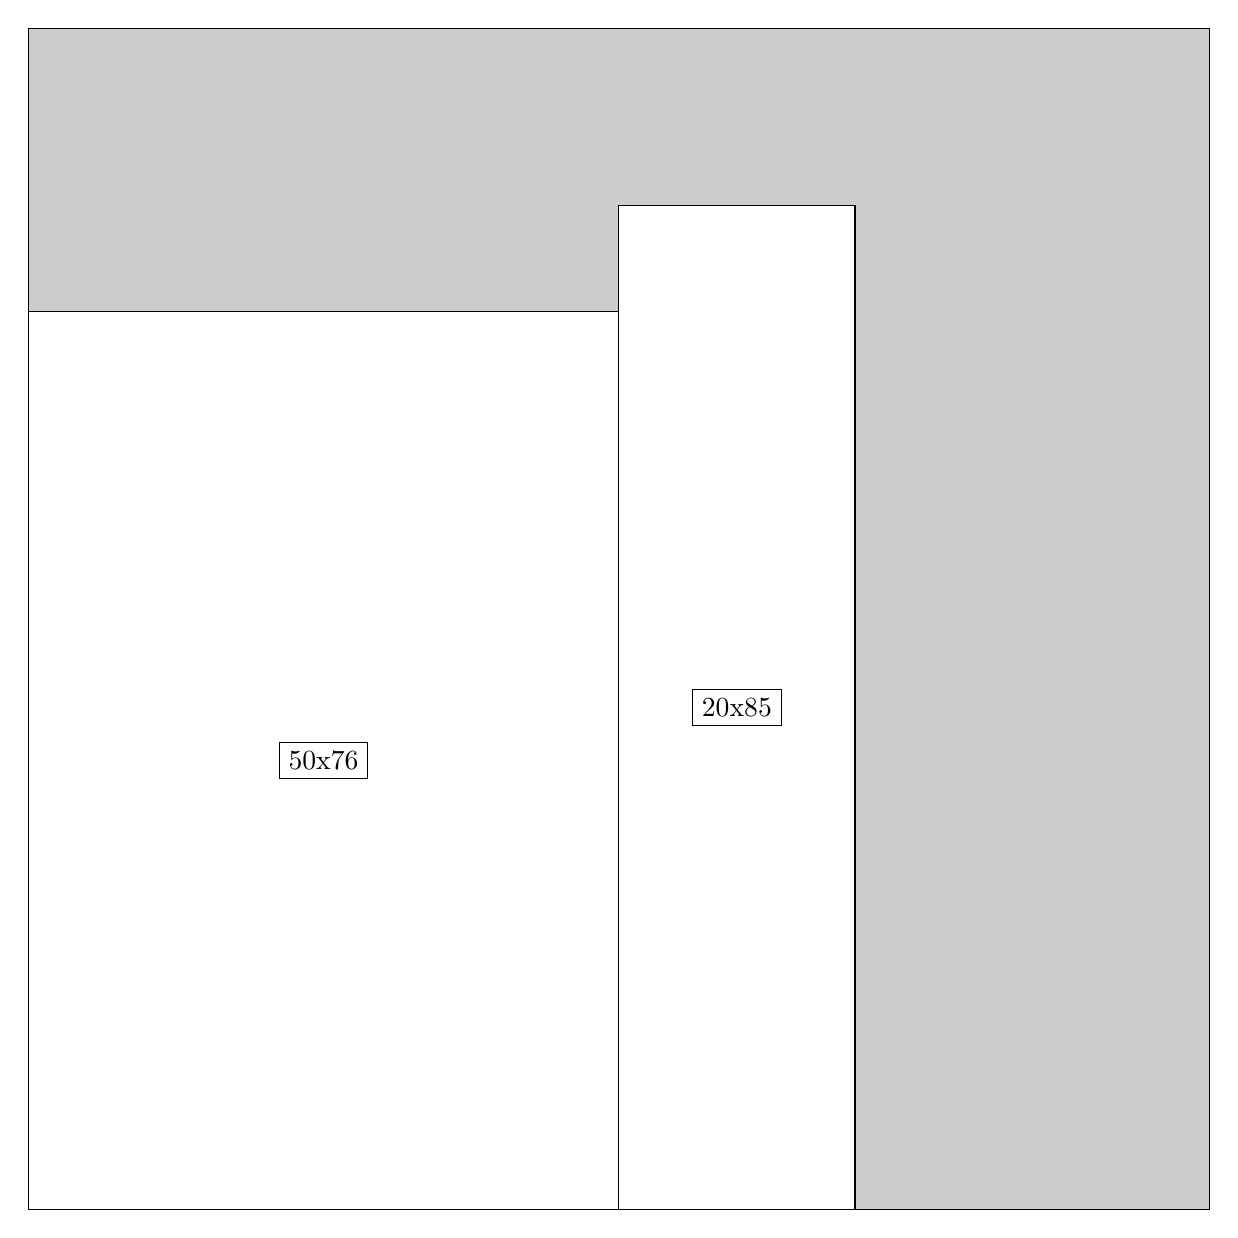
\begin{tikzpicture}[shorten >=1pt,scale=1.0,every node/.style={scale=1.0},->]
\tikzstyle{vertex}=[circle,fill=black!25,minimum size=14pt,inner sep=0pt]
\filldraw[fill=gray!40!white, draw=black] (0,0) rectangle (15.0,15.0);
\foreach \name/\x/\y/\w/\h in {20x85/7.5/0.0/3.0/12.75,50x76/0.0/0.0/7.5/11.4}
\filldraw[fill=white!40!white, draw=black] (\x,\y) rectangle node[draw] (\name) {\name} ++(\w,\h);
\end{tikzpicture}


w =20 , h =85 , x =50 , y =0 , v =1700
\par
w =50 , h =76 , x =0 , y =0 , v =3800
\par
\newpage


\end{document}